\documentclass{mul_poster}

\usepackage[utf8]{inputenc}

\begin{document}

\title{\parbox{0.95\paperwidth}{Defects and their influence on mechanical properties in nitrides: an atomistic study}}
\author{Betreuer: David Holec}
\authorPhoto{figs/lukas}
  {\centering Lukas Löfler\\11/2017 -- 07/2022}
\makeHeader

\node[below left] at (1\textwidth, 1\textheight) {\includegraphics[width=5cm]{graphics/logo_tuw}};
\node[above right] at (0, -1) {
\includegraphics[width=8cm]{graphics/logo_fwf}};
\node[above left] at (\textwidth, -1) {
\includegraphics[height=3cm]{graphics/logo_vsc}};


\posterBox*{1.7}(0.3,-7.3){Motivation}{
  Transition metal nitride-based coatings are a common choice when thinking about protective coatings. They have high hardness, good resistance against mechanical wear and are both chemically and thermally stable. In order to create improved coatings, one can, next to alloying, carefully introduce defects into the system. Defects, ranging from vacancies to grain boundaries, can heavily alter the behaviour of a material. One way to use defects is to create multilayered coatings, introducing numerous interfaces which can be considered as a defect. It was shown that an increase in both hardness and fracture toughness can be reached in multilayered coatings consisting of alternating layers of two different materials. To get a better understanding of the role of the interface in such coatings, atomistic simulations, in the form of density functionality and classical molecular dynamics, were performed to investigate the influence of defects on mechanical properties. The main focus is on multilayered systems; here, the impact of both interface and magnetic configurations was studied in CrN-based systems. Further, \textit{in silico} mechanical experiments in the form of tensile loading and nanoindentation of AlN/TiN multilayers were performed.
}

\posterBox*{2}(0,0){Simulations}{  
  \begin{minipage}{0.48\textwidth}
    \begin{itemize}
      \item The classical molecular dynamics simulations were run with the LAMMPS package.
      \item The atomic interactions were described by an AlTiN MEAM potential. 
      \item Tensile loading and nanoindentation \textit{in silico} experiments were performed on AlN/TiN  multilayers with layer thicknesses $\Lambda =$ 1.25, 2.5, 5 and 10\,nm.
    \end{itemize}
  \end{minipage}
  \hfill
  \begin{minipage}{0.5\textwidth}
    \begin{itemize}
      \item Density Functional Theory (DFT) calculations performed with the VASP package. 
      \item PAW pseudopotentials with GGA-PBE exchange correlation described the interactions.
      \item The fracture toughness of AlN/CrN and TiN/CrN was simulated for different interfaces and magnetic configurations.
    \end{itemize}
  \end{minipage}
}

 \posterBox*{1}(0,5){Tensile loading of AlN/TiN}{
  \begin{itemize}
    \item AlN/TiN multilayers with various $\Lambda$ were strained $\|$ and $\perp$ to the interface.
    \item In-plane loading shows a dependence on the layer thickness with an increased toughness for smaller layer thicknesses.
    \item AlN exhibits a phase transformation from the initial B1 structure towards B3 and B4 structures under tensile loading.
    \item Areas of phase transformations have $\wedge$ and $\vee$ shape (see figure below), leading to local stress concentrations, decoherence of the interfaces and, consequently, failure.
    \item Under $[110]$-tension, layers start to slip at an 45$^\circ$ angle to the interface.
  \end{itemize}\bigskip
  \centering
  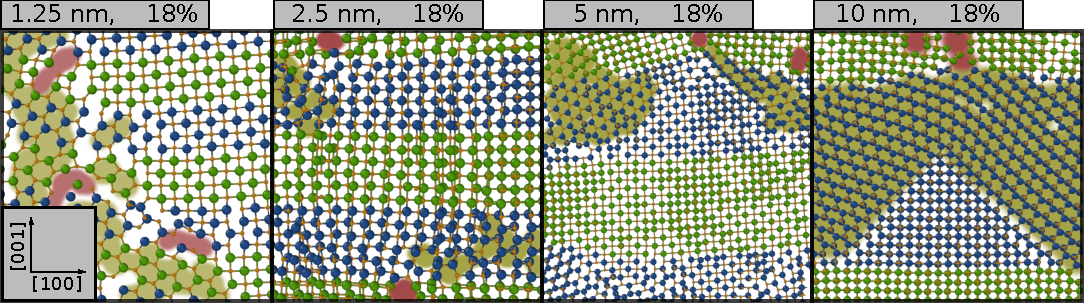
\includegraphics[width=\textwidth]{figs/100_struc_change.pdf}\bigskip\\
  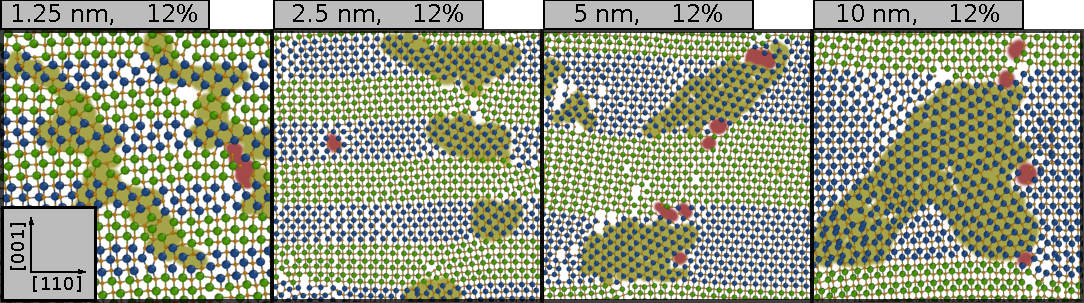
\includegraphics[width=\textwidth]{figs/110_struc_change.pdf}\\
  {\small Phase transformation (yellow) and failure (red) AlN(blue)/TiN(green) multilayers, strained along the [100]- (top) and [110]-direction (bottom) $\|$ to the interface. Red areas highlight broken bonds serving as nucleation sites for cracks.}
}

\posterBox*{1}(1,5){Indentation of AlN/TiN}{
  \begin{itemize}
    \item Indentation of AlN/TiN reveals intermixing of the individual layers driven by shear stresses. 
    \item The composition in the intermixing zone converges towards the ratio between the two layer thicknesses. 
    \item Dislocations growth starts to increase with the onset of intermixing.
    \item For initial hardness, the top layers should be of the individually harder material (TiN in this case).
    \item Loading along the $[110]$ direction, $\|$ to the interface, leads to a slip of layers, a behaviour also found in TEM investigations of AlN/TiN thin films after nanoindentation.
  \end{itemize}\medskip
  \centering
  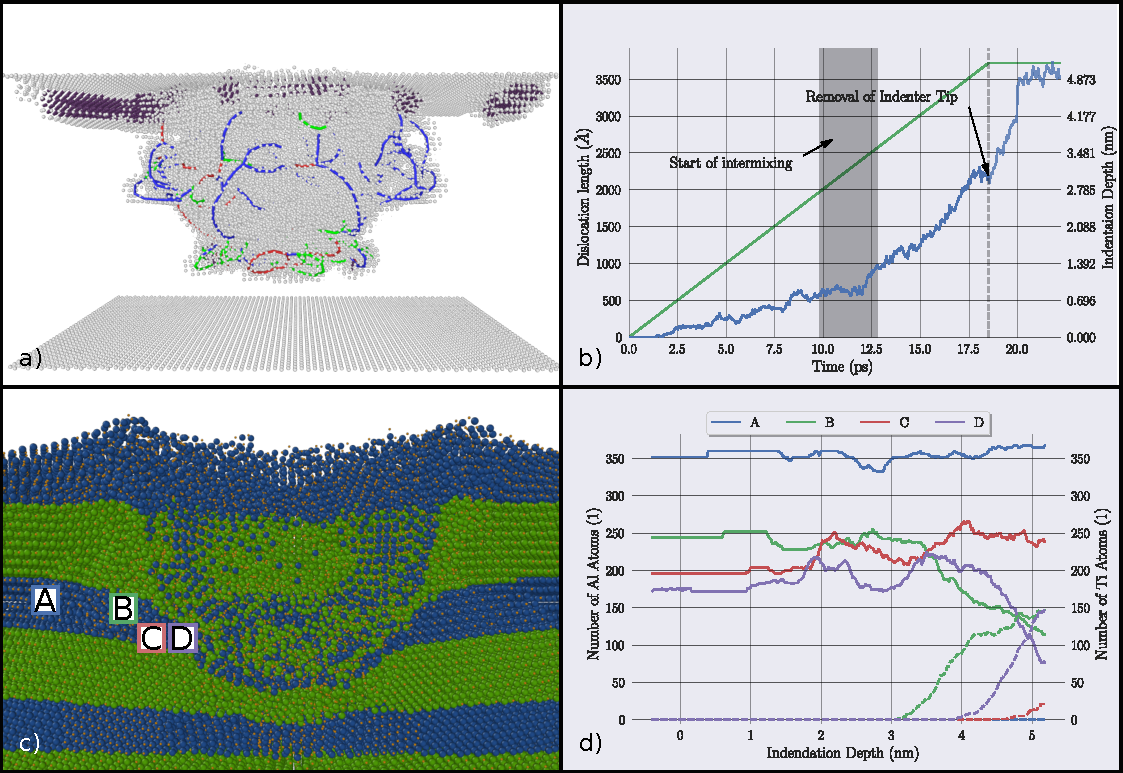
\includegraphics[width=0.9\textwidth]{figs/disloc_and_mixing.pdf}\\
  {\small Indentation AlN(blue)/TiN(green) multilayers normal to the $[001]$ interface.}
}

\posterBox*{2}(0,25.8){Interfaces and magnetism in AlN/CrN and TiN/AlN}{
  \begin{minipage}{0.50\textwidth}
    \centering
    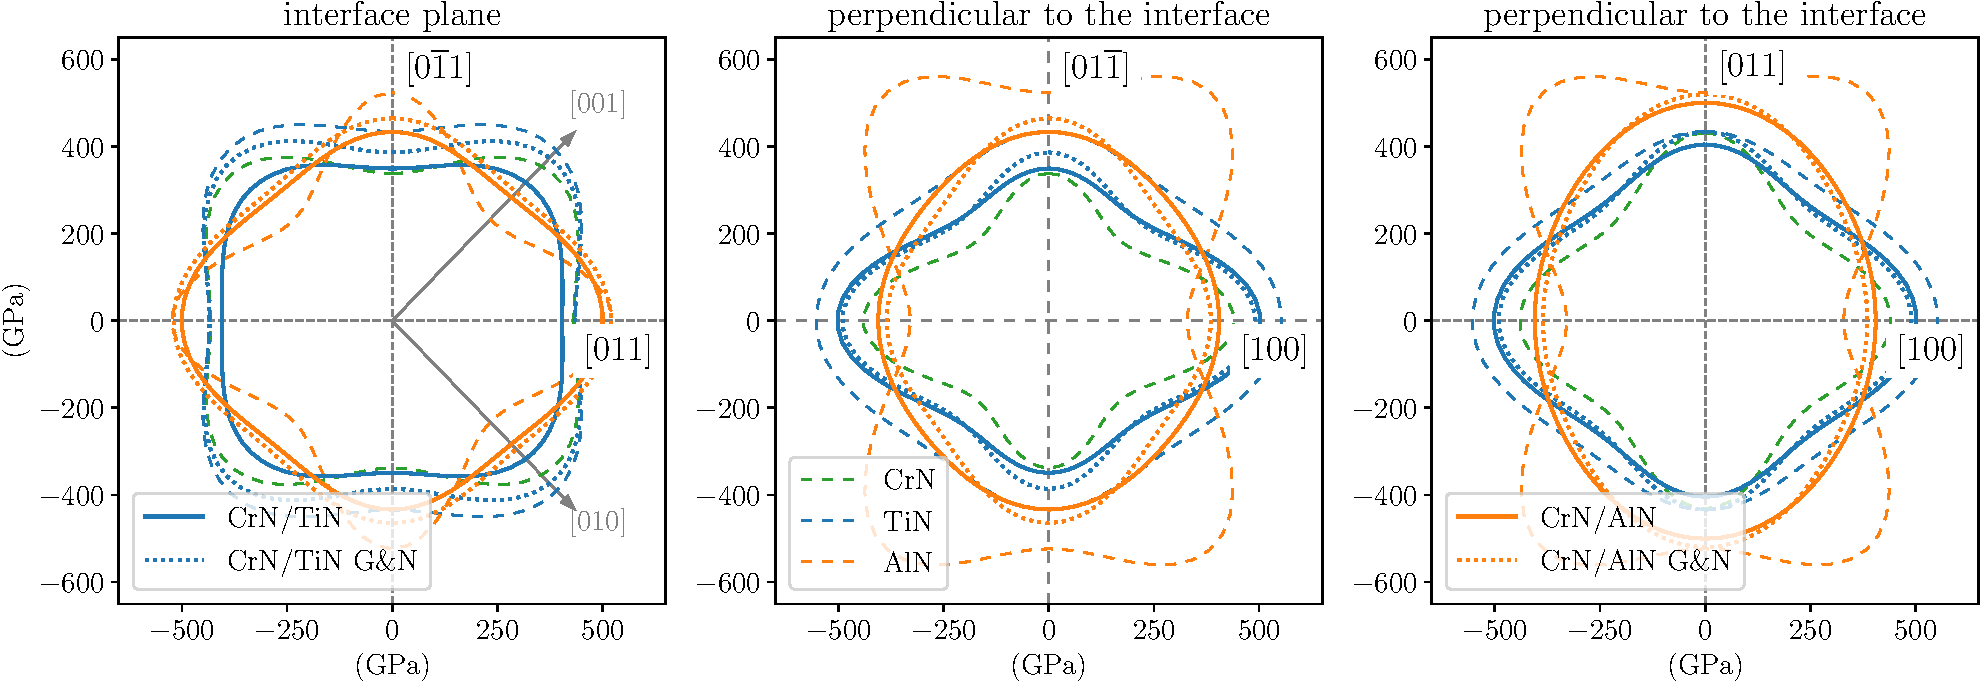
\includegraphics[width=0.9\textwidth]{figs/E_modul_100-crop.pdf}\\
    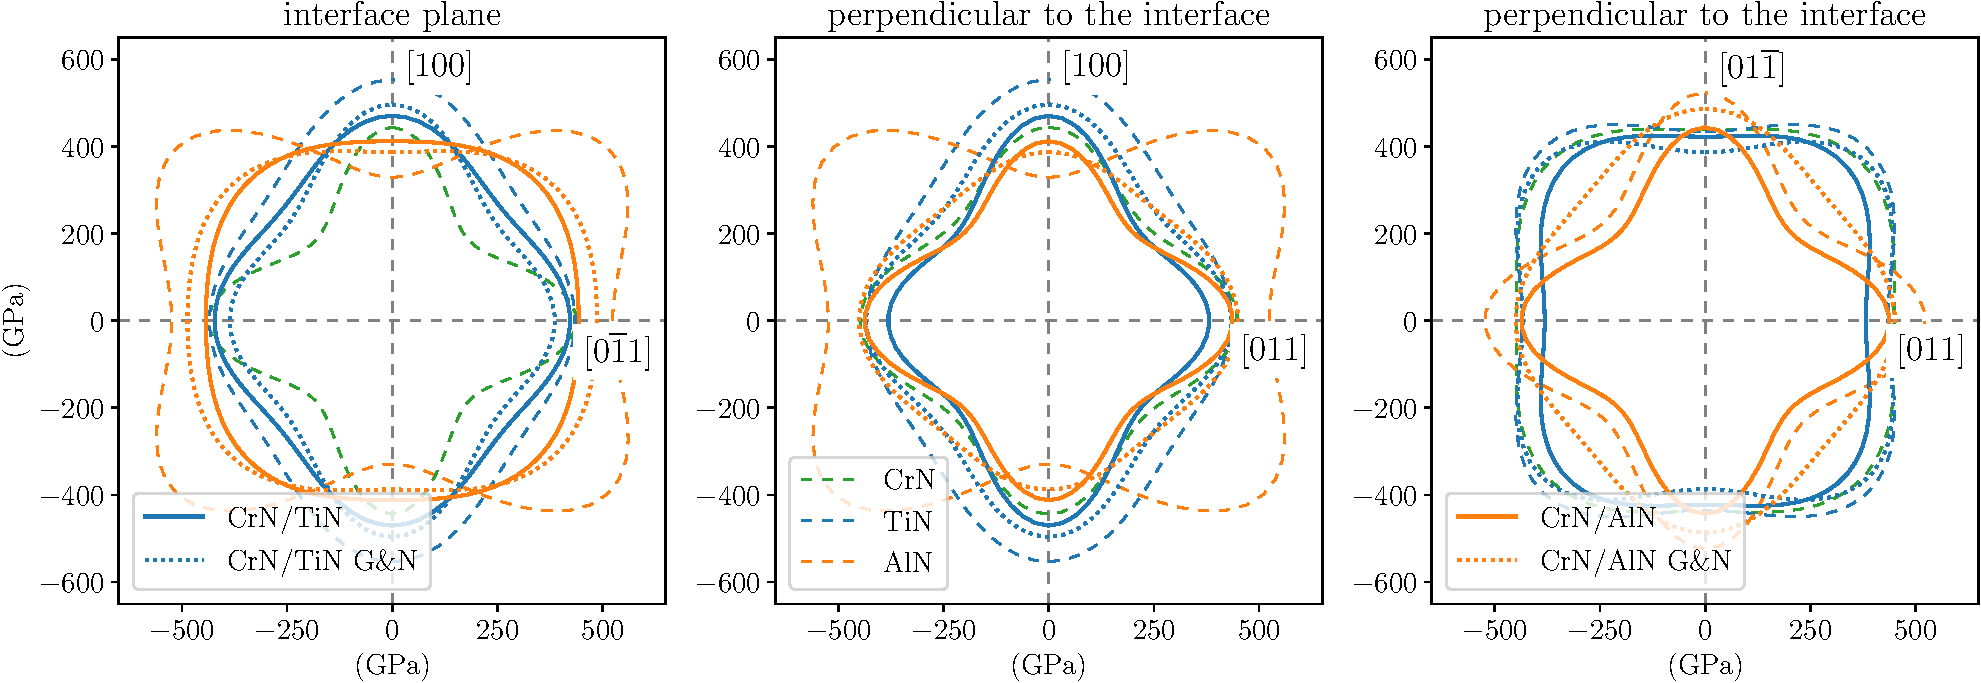
\includegraphics[width=0.9\textwidth]{figs/E_modul_011-crop.pdf}\\
    {\small Directional Young's moduli of afm AlN/CrN and TiN/CrN multilayers with [100] interface (top) and [110] interface (bottom) in comparison with the values of the binary systems as well as the values obtained with the Grimsditch and Nizzoli method.}
  \end{minipage}\quad
  \begin{minipage}{0.48\textwidth}
    \begin{minipage}{\textwidth}
      \begin{itemize}
        \item The influence of both the interface orientation and magnetic configuration in AlN/CrN and TiN/CrN multilayers was studied using DFT.
        \item The layered structure has no impact on the local magnetic moments. 
        \item In many cases, the efficient continuum-mechanics-based approach of Grimsditsh and Nizzoli brings good results; the interface should, however, be considered explicitly as it could be essential to describe the elastic behaviour correctly.     
        \item The ferromagnetic configuration is not suitable to substitute for anti-ferro- and paramagnetic configurations.
      \end{itemize}
    \end{minipage}\bigskip\\
    \begin{minipage}{\textwidth}
      \begin{minipage}{0.65\textwidth}
        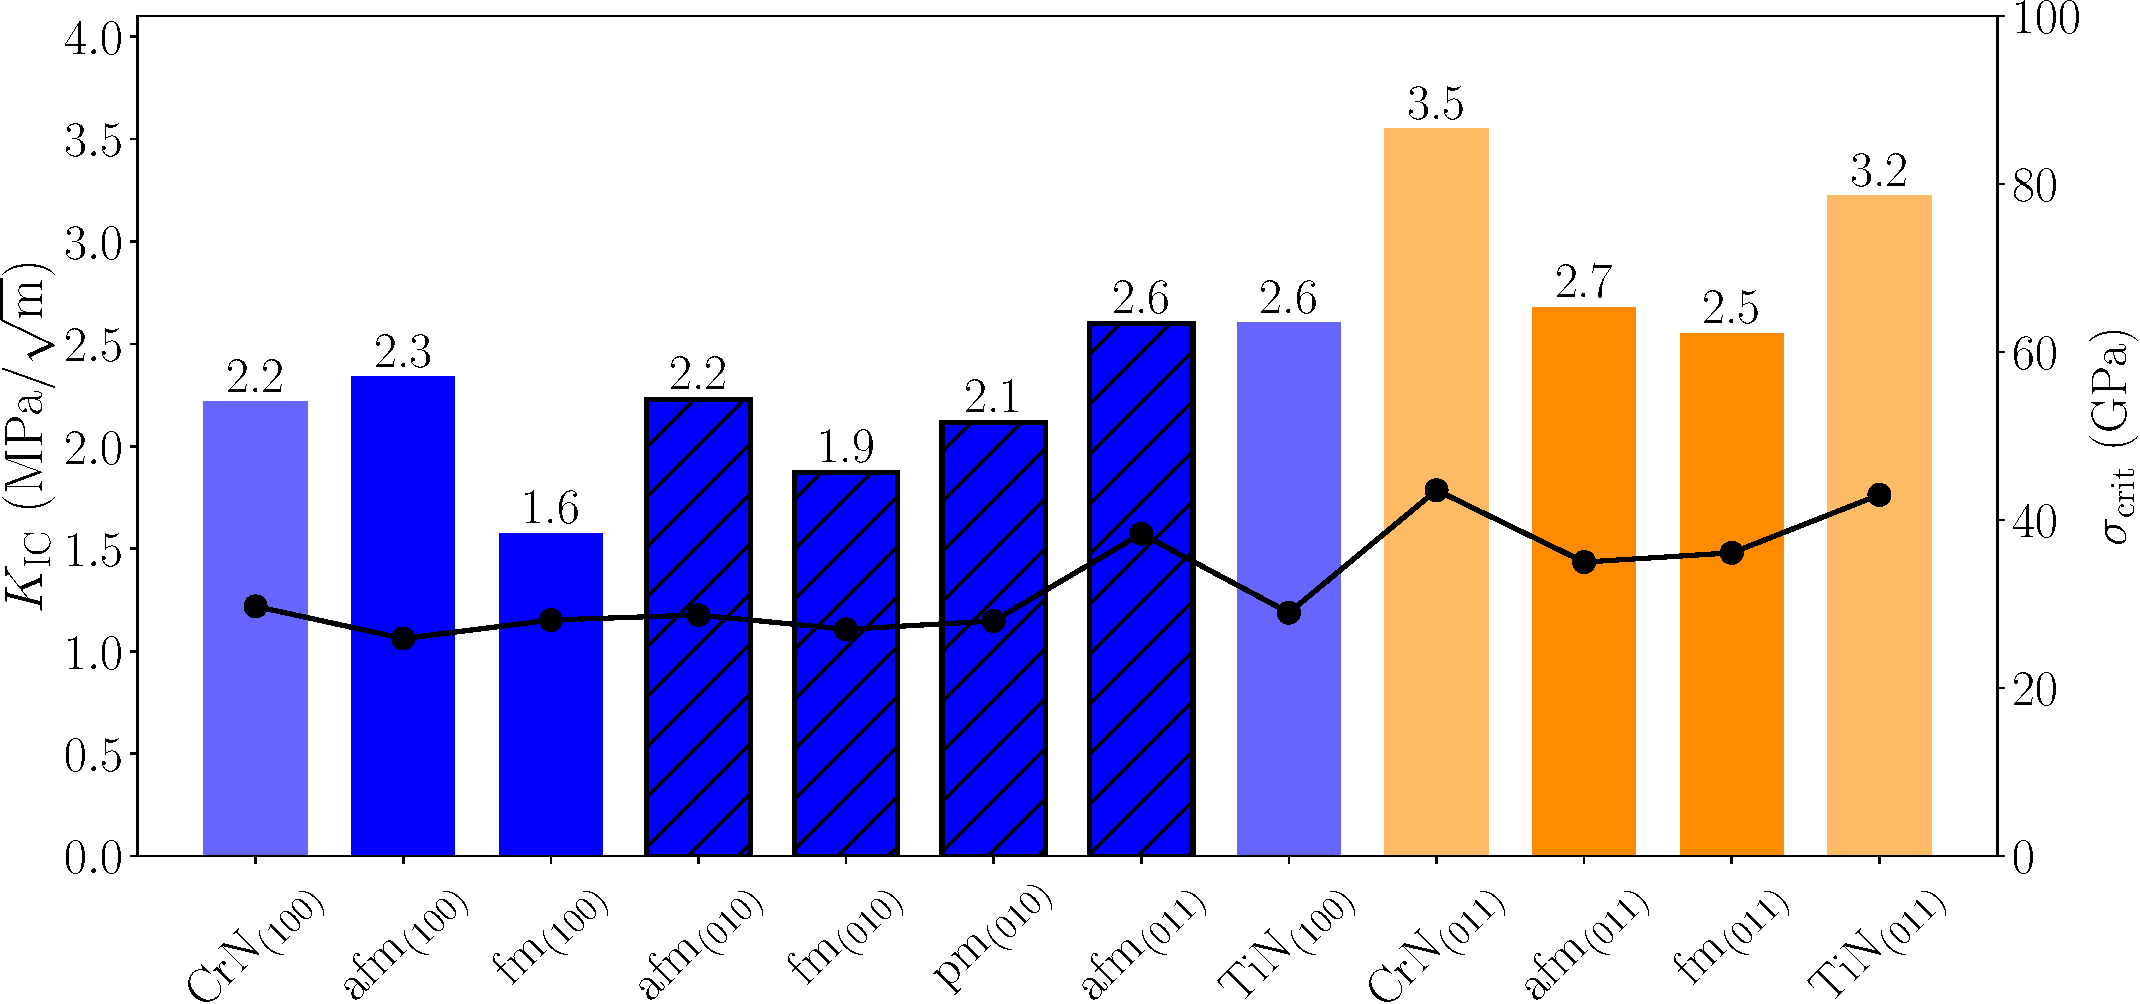
\includegraphics[width=\textwidth]{figs/kic_CrN_TiN-crop.pdf}\\
        {\small Fracture toughness ($K_{IC}$) for TiN/CrN with [100] (blue) and [110]-interface (orange) and the critical stress ($\Sigma_\mathrm{crit}$, black line). The full plain bars denote cleaving $paralell$ the hatching bars cleaving $\perp$ to the interface.}
      \end{minipage}
      \hfill
      \begin{minipage}{0.32\textwidth}
        \begin{itemize}
          \item The fracture toughness was determined by: $$K_{IC} = \sqrt{2 \pi E \gamma}\ ,$$ utilising the directional Young's moduli ($E$) and substituting the surface energy ($\gamma$) with the cleavage energy. 
          \item The critical stress (at $l_\mathrm{crit}$) gives an indication of the strength of the bonds at the plane of cleavage. 
        \end{itemize}
      \end{minipage}
    \end{minipage}
 \end{minipage}
}

\node[above] at (0.5\textwidth, 2.5) {
  \small
  {\bfseries Acknowledgements:} The work was funded by the Austrian Science Fund (P 30341-N36). The computational results presented have been achieved using the Vienna Scientific Cluster (VSC).
};
\end{document}
